%=============================================================
\chapter{Motivation}
\label{ch:motivation}
%=============================================================

This thesis focuses on disk-based ANNS under concurrent on-premise serving.
In this setting, the vector index is too large to fit fully in DRAM and must be stored on SSD, while many users and agents issue retrieval requests to the same machine.
The bottleneck is therefore not only the latency of a single SSD read, but the interaction between random I/O, high concurrency, and fixed-budget graph search.

PaceANN is motivated by three observations.
First, NVMe latency grows nonlinearly once the effective queue depth passes the device's knee.
Second, DiskANN beam search often continues expanding after the top-$k$ result has already converged.
Third, these unnecessary reads amplify tail latency because all concurrent queries share the same SSD queue.

%-------------------------------------------------------------
\section{Nonlinear Queueing Latency on NVMe SSDs}
\label{sec:mot-ssd}
%-------------------------------------------------------------

Disk-based ANN search is dominated by random SSD reads\cite{ren2025storageann}.
Figure~\ref{fig:fio-qd} shows a 4\,KB random-read \texttt{fio} scan on our NVMe SSD using both \texttt{libaio} and \texttt{io\_uring}.
The two interfaces produce nearly identical curves, indicating that the main effect comes from the device queue rather than the submission API.

\begin{figure}[htbp]
  \centering
  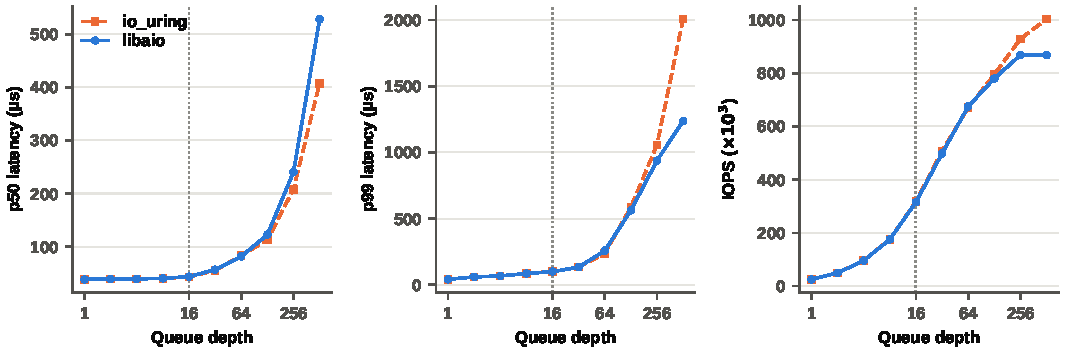
\includegraphics[width=\textwidth]{img/fio_qd_3panel.pdf}
  \caption[NVMe SSD latency and IOPS versus queue depth]{p50 latency, p99 latency, and IOPS of our NVMe SSD under single-threaded 4\,KB \texttt{O\_DIRECT} random reads as queue depth increases, comparing \texttt{io\_uring} and \texttt{libaio}. Latency remains nearly flat until QD~$\leq$~16 (dashed line), then rises sharply. IOPS growth slows substantially after QD~$\approx$~256 and approaches saturation.}
  \label{fig:fio-qd}
\end{figure}

Latency stays almost flat until QD~$\leq$~16, then rises sharply, while IOPS approaches saturation around QD~$\approx$~256.
After the knee, extra in-flight requests mainly add queueing delay rather than increasing useful throughput.
In a concurrent server, the SSD observes the aggregate queue depth across workers, $D_\text{eff}=\sum_t D_t$.
With 32 workers and beam width 8, the worst case can reach about 256 in-flight reads, far beyond the latency knee.
Thus, reducing unnecessary reads is a direct way to lower queueing delay for all queries.

%-------------------------------------------------------------
\section{Diminishing I/O Benefit in Beam Search}
\label{sec:mot-diminishing}
%-------------------------------------------------------------

DiskANN beam search gains most of its useful information in the early hops.
Later hops often explore nodes near the already discovered neighborhood and rarely change the final top-$k$ result.
To quantify this, we run an oracle early-termination analysis on SPACEV100M.
For each query, we record the top-$k$ after every hop and find the earliest hop $h^*$ that reaches the final recall of the full search.
Hops after $h^*$ are treated as wasted post-convergence work.

\begin{table}[h]
\centering
\caption[Oracle early-termination analysis on SPACEV100M]{Oracle early-termination analysis on SPACEV100M for different $L$ values ($W = 8$, $K = 10$). All columns report per-query averages over the query set.}
\label{tab:oracle-summary}
\begin{tabular}{rrrrr}
\hline
$L$ & Mean actual hops $\bar h_\text{total}$ & Mean oracle hops $\bar h^*$ & Wasted hops\,\% & Recall@10 \\
\hline
 20 &  9.2 &  8.6 &  6.8\% & 0.897 \\
 60 & 13.6 &  9.3 & 31.5\% & 0.955 \\
100 & 18.4 &  9.8 & 46.7\% & 0.968 \\
150 & 24.4 & 10.3 & \textbf{57.8\%} & 0.977 \\
200 & 30.4 & 10.6 & 65.1\% & 0.981 \\
\hline
\end{tabular}
\end{table}

The wasted fraction increases as the target recall rises.
At $L=150$, the search executes 24.4 hops on average, while the oracle needs only 10.3 hops to reach the same final recall.
This means 57.8\% of hops occur after convergence.
At $L=200$, the wasted fraction reaches 65.1\%.
Because each hop can issue up to $W$ SSD reads, post-convergence expansion creates substantial avoidable I/O.

This also shows why a single global $L$ is inefficient.
Easy queries converge quickly, while difficult queries need a larger budget.
Using one fixed budget forces easy queries to pay for the worst cases.
A per-query stopping rule is therefore more appropriate for concurrent serving.

%-------------------------------------------------------------
\section{Amplification of Ineffective I/O in Concurrent Servers}
\label{sec:mot-tail}
%-------------------------------------------------------------

The SSD queueing effect and the wasted-hop effect reinforce each other.
I/O from post-convergence hops keeps $D_\text{eff}$ high, and high $D_\text{eff}$ increases the latency of both useful and useless reads.
This is especially harmful for tail latency, because a few queries can encounter congestion peaks and delay the workers serving later requests\cite{dean2013tail}.

Existing systems optimize different parts of this cost.
Starling improves the usefulness of each page read through layout changes\cite{wang2024starling}, while PipeANN overlaps computation and I/O to hide part of single-query latency\cite{osdi25pipeann}.
PaceANN instead reduces the number of reads that enter the shared SSD queue.
This is the main lever for improving throughput and P99 latency when the SSD is already operating beyond its queue-depth knee.

%-------------------------------------------------------------
\section{Key Insight: Convergence Can Be Detected Without Extra I/O}
\label{sec:mot-insight}
%-------------------------------------------------------------

The key requirement is to detect convergence without issuing more SSD reads.
DiskANN already keeps PQ-compressed codes in memory, so it can estimate distances to unexpanded candidates using only CPU computation.
For expanded candidates, the full-precision vectors have already been read, so exact distances are available.
Before each hop, PaceANN can compare the best unexpanded candidate's PQ estimate with the exact-distance boundary of the current result set.
If the frontier is unlikely to improve the top-$k$, the query can stop.

This signal is more reliable once the early search state has enough coverage.
PAC helps by keeping frequently visited early nodes in DRAM, while CA-ET removes later hops after convergence.
The two mechanisms therefore support the same goal: reduce avoidable SSD I/O without changing the underlying DiskANN index.
